\def\reverse{$\mathop{\mathit{reverse}}(i, j)$}
\def\Bp{$\hbox{\rm B}^+$}

\section{Vyvážené stromy}

Pôvodná verzia \citep{kuko} obsahovala vizualizáciu viacerých vyvážených stromov.
K nim sme pridali \Bp-stromy, stromy s prstom a stromy s reverzami.

\subsection{B$^+$-strom}

\paragraph{Popis.}
\emph{\Bp-strom} je variácia B-stromu, v ktorom sú všetky kľúče uložené v listoch
a listy sú pospájané do spájaného zoznamu. \Bp-strom rádu $B$ je strom, v ktorom
má každý vnútorný vrchol najmenej $\lfloor B/2 \rfloor$, ale najviac $B$ synov.
Vďaka tomu je dobre vyvážený a jeho operácie sú vykonávané v logaritmickom čase.
\Bp-strom je \emph{asociatívne pole (slovník)}, čiže poskytuje tieto tri operácie:
\begin{itemize}
\item $\ins(x)$ -- pridá do stromu $x$;
\item $\find(x)$ -- zistí, či sa v strome nachádza $x$;
\item $\delete(x)$ -- odstráni zo stromu $x$.
\end{itemize}

Operácia $\find$ začne v koreni, nájde v ňom prvý kľúč väčší od hľadaného.
Nech je $i$-ty v poradí, potom hľadanie pokračuje v $i$-tom synovi tohto vrcholu.
Je zrejmé, že ak sa väčší kľúč nenájde, presunieme sa do posledného, $B$-tého syna.
V liste sa už len skontroluje, či sa v ňom hľadaný kľúč nachádza.

Definujeme dve operácie: {\sc Copy-Up} a {\sc Push-Up}, ktoré používa operácia $\ins$.
Ak má vrchol viac prvkov, ako je maximálny limit, treba ho zmenšiť. Rozdelí sa na dve časti.
Ak vrchol nie je listom, použije sa {\sc Push-Up}, najmenší kľúč pravej časti sa vyberie
a stane sa otcom vytvorených dvoch častí. Pokiaľ to list je, kľúč v ňom musí zostať,
preto sa iba skopíruje. Táto operácia sa nazýva {\sc Copy-Up}.

Operácia $\ins$ najprv pomocou operácie $\find$ zistí, či štruktúra daný kľúč obsahuje.
Ak nie, je zrejmé, že patrí práve do vrchola, kde $\find$ skončil. Ak má vrchol po vložení
viac kľúčov ako maximálny limit, je treba ho zmenšiť. Pokiaľ otcovský vrchol má syna,
do ktorého je možné kľúč presunúť a zároveň syn susedí s veľkým vrcholom, postup je nasledovný.
Nech je vrchol vľavo menší a terajší vrchol je $i$-ty syn v poradí. Potom algoritmus z neho
vyberie najmenší kľúč, presunie ho na miesto $(i-1)$-ho kľúča v otcovskom vrchole. Vymenený
kľúč následne vloží do $(i-1)$-ho syna. Ak sú susedné vrcholy príliš veľké na presun kľúča,
použije sa operácia {\sc Copy-Up}. Nový vrchol s jedným kľúčom, ktorý vznikol, vložíme do
otcovského vrcholu. Ak otcovský vrchol presiahol najväčšiu možnú veľkosť, znova sa aplikuje
popísaný algoritmus s jedným rozdielom -- namiesto {\sc Copy-Up} sa použije {\sc Push-Up}.

Operácia $\delete$ najprv pomocou $\find$ nájde kľúč, potom ho z vrcholu odstráni. Tento vrchol
môže mať po odstránení menší počet kľúčov ako minimálny limit. Vtedy, ak sa dá, sa prenesie
jeden kľúč zo súrodenca. Ak sa nedá, vrchol sa s ním zlúči. Zároveň sa k nim pridá aj kľúč
z otcovského vrcholu, ktorý ich rozdeľoval. Pokiaľ to spôsobilo, že otcovský vrchol má menej
kľúčov, ako je povolené, znova sa aplikuje predošlý algoritmus. Keďže na koreň sa nevzťahuje
minimálny limit, po skončení bude strom zaručene v konzistentnom tvare.

%\paragraph{Časová zložitosť}
%\todo{toto je pocet pristupov na disk! pocet krokov je $O(B\log_B n)$; ale pocet pristupov
%na disk nas zaujima, lebo disk je pomaly}
Vkladanie, vymazávanie a hľadanie má časovú zložitosť $O(\log_B n)$.

\paragraph{Použitie.}
Hlavné využitie \Bp-stromov je v databázových systémoch. Ak zvolíme vhodný rád, vieme jednotlivé
vrcholy dobre napasovať na stránky a tým regulovať ako počet prístupov k pamäti, tak jej zaplnenie
\citep{sahni}. Agregačné funkcie, ako napríklad súčet, minimum, priemer, vieme pre daný interval
spočítať v čase $O(\log_B(n))$. Vypísať všetky prvky z daného intervalu dokážeme pomocou
$O(\log_B(n) + t/B)$ prístupov na disk.
% \Bp-strom podporuje efektívne vyhľadanie prvkov poľa, ktoré patria do daného intervalu.
% Algoritmus nájde jeden krajný bod a vďaka spájanému zoznamu, vytvorenému z listov, ostatné prvky
% postupne prečíta. Zložitosť je $O(\log_B(n) + t/B)$, kde $t$ je počet výsledných kľúčov z hľadaného intervalu.

Ďaľšia výhoda \Bp-stromov oproti B-stromom sa prejaví, ak máme utriedený zoznam dát a chceme z neho vytvoriť \Bp-strom:
\Bp-strom môžeme vystavať odspodu. Takýto postup nám zaručí vyžaduje $O((n/B)\cdot\log_B n)$ prístupov na disk,
čo je $B$-krát rýchlejšie ako spraviť $n$ volaní $\ins$.




\subsection{Strom s prstom}
\emph{Strom s prstom} (z anglického Finger tree) je vyhľadávací strom s hranami na vrstvách a štruktúrou 
nazývanou prst. Prst je smerník na konkrétny vrchol a umožňuje (aj vďaka väzbám navyše) efektívnejší 
prístup k vrcholom v jeho blízkom okolí.

\paragraph{Popis.}
Strom s prstom je upravený 2-3-4$^+$ strom (\Bp-strom rádu 4, t.j.\ vnútorné vrcholy
majú stupeň 2, 3 alebo 4). Kľúče sú uložené v listoch a vnútorné vrcholy
obsahujú ich kópie, aby viedli vyhľadávanie. Pre podporu vyhľadávania
s prstom spojíme všetky vrcholy na rovnakej úrovni (v rovnakej vzdialenosti od koreňa)
do obojsmerného spájaného zoznamu.
Ak sú nejaké dva vrcholy spojené takouto hranou, budeme hovoriť, že sú susedia.

Prst, ako už bolo spomenuté, ukazuje na nejaký vrchol. Môže sa pohybovať po všetkých hranách
a pomocou neho sa vykonávajú všetky operácie. Keďže sú všetky kľúče uložené v listoch, prst
na tejto vrstve začína, aj končí.

Vzhľadom na usporiadanie budem predpokladať, že menšie prvky sa nachádzajú vždy vľavo a každý
prekopírovaný kľúč má svoj originál vždy vľavo v listovom vrchole.

% Strom s prstom je \emph{asociatívne pole (slovník)}, čiže
% poskytuje tieto tri operácie:
% \begin{itemize}
% \item $\ins(\k)$ -- pridá do stromu $\k$;
% \item $\find(\k)$ -- zistí, či sa v strome nachádza $\k$;
% \item $\mathop{\mathbf{delete}}(\k)$ -- odstráni zo stromu $\k$.
% \end{itemize}

Operácia $\find$ začne na mieste, kam ukazuje prst. Skontroluje, či by kľúč mal patriť do daného
vrcholu. Ak nie, pozrie sa, či nepatrí do niektorého zo susedov. Ak áno, prst sa tam presunie
a vyhľadávanie sa skončilo. Inak smerník prejde o vrstvu vyššie, na otcovský vrchol. Ak hľadaný
kľúč patrí do jeho podstromu (t.j.\ je väčší ako jeho najmenší kľúč a menší ako ten najväčší),
zíde po hranách do listu, kde by sa daný kľúč mal nachádzať. Keď do podstromu nepatrí, skontroluje,
či nepatrí do podstromu susedov. Ak áno, prejde po vrstevnej hrane na suseda a následne zíde až
do listu, kde by mal kľúč byť. Pokiaľ prst nenarazil na správny podstrom, znova sa presunie smerom
nahor po otcovskej hrane. Hľadanie pokračuje analogicky. Je zrejmé, že ak prst ukazuje na koreň,
kľúč bude patriť do jeho podstromu.

% Otázka patričnosti do podstromu sa dá pre krajné prípady optimalizovať. Ak totiž vrchol, na ktorý
% ukazujeme, nemá napríklad pravého suseda, je zrejmé, že vačší kľúč ako je najvačší v tomto vrchole
% v strome nie je. Preto ľubovoľný kľúč do podstromu tohto vrchola patrí práve vtedy, keď je väčší
% ako jeho najmenší prvok. Analogicky to platí, ak chýba ľavý sused.

% <<<<<<< HEAD
% Operácia \ins\ najprv pomocou operácie \find\ nájde miesto, kam by mal vkladaný kľúč patriť. 
% Ak taký kľúč už v strome je, ďalší sa nevloží. V prípade, že sme vložili nový kľúč, môže sa stať, 
% že vrchol "pretečie", tzn.\ má viac ako 3 prvky%
% (pozri obr.~\ref{img:finger-insert}). Situácia sa vyrieši rovnako ako v \Bp-strome. 
% 
% Operácia \delete\ najprv pomocou operácie \find\ nájde miesto, kam by mal hľadaný kľúč patriť. 
% =======
Operácia $\ins$ najprv pomocou operácie $\find$ nájde miesto, kam by mal vkladaný kľúč patriť.
Ak taký kľúč už v strome je, ďalší sa nevloží. V prípade, že sme vložili nový kľúč, môže sa stať,
že vrchol "pretečie", tzn.\ má viac ako 3 prvky. Situácia sa vyrieši rovnako ako v \Bp-strome.
Operácia $\delete$ najprv pomocou operácie $\find$ nájde miesto, kam by mal hľadaný kľúč patriť.
% >>>>>>> a0feba993f87ff1223dad61de4a624b8b4102adb
Ak tam nie je, vymazávanie sa končí. Inak sa vymaže. Môže sa stať, že vrchol "podtečie", tzn.\ 
nemá kľúč. Tento problém sa rieši rovnako ako v \Bp-strome. 
Samozrejme je treba ošetriť konzistentnosť vo vyšších vrstvách, aby sa tam nenachádzali kópie 
kľúčov, ktoré už boli zo štruktúry vymazané (pozri obr. ~\ref{img:finger-delete}).  

\begin{figure}
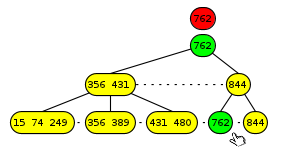
\includegraphics[width=\columnwidth]{obrazky/finger-delete.png}
\caption{\emph{Vymazávanie kľúča $762$.} Odstrániť sa musí aj kópia vo vyšších vrstvách.}
\label{img:finger-delete}
\end{figure}

\begin{figure}
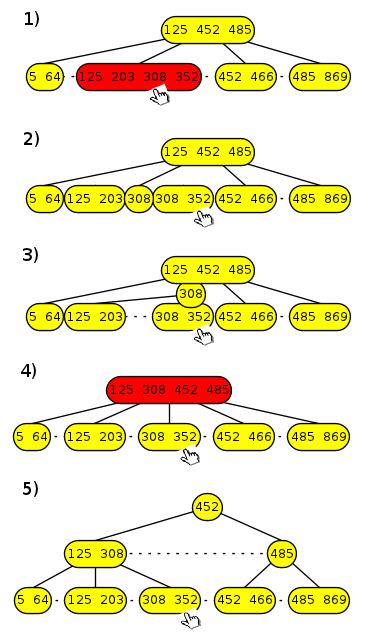
\includegraphics[width=\columnwidth]{obrazky/finger-insert.png}
\caption{\emph{Pretečenie vrchola.} Do stromu sme vložili prvok $308$ a 1) listový vrchol pretiekol. 
2) vrchol sa delí a kľúč sa kopíruje, aby originál zostal v liste 3) nový otec sa vkladá do vyššej vrstvy 
4) aj tento vrchol preteká, delí sa a vzniká nový koreň 5) finálny tvar.}
\label{img:finger-insert}
\end{figure}

\paragraph{Časová zložitosť.}
Keďže každý vrchol má aspoň dvoch synov, 2-3-4 strom má hĺbku $O(\log n)$, kde $n$ je počet kľúčov, 
a teda podporuje vykonávanie operácií v čase $O(\log n)$. Ak sa však použije prst, časová zložitosť 
vychádza na $O(\log d)$, kde $d$ je vzdialenosť pozície prsta a vrcholu, kam patrí cieľový kľúč, 
amortizovane dokonca na $O(1)$ \citep{sahni}. 

% \paragraph{Použitie.}
% Prst ako smerník na prvok štruktúry, ktorý umožňuje efektívnejší prístup k okolitým kľúčom, prvýkrát
% spomenuli Guibas et al. Vo svojej publikácii prezentujú B-strom podporujúci vyhľadávanie v $O(\log n)$
% a update-y dokonca v $O(1)$ čase, predpokladajúc, že je udržiavaných len $O(1)$ pohyblivých prstov \citet{sahni}.
% Pohyb prsta o $d$ pozícií trvalo $O(\log n)$ času. Na základe tejto práce navrhli Huddleston a Mehlhorn
% svoj vrstvovo spájaný 2-3-4 strom, ktorý bol neskôr upravený vďaka Belloch et al. na priestorovo efektívnejšiu
% alternatívu. Toto riešenie využíva jeden prst, s ktorým štruktúra ponúka rovnakú operačnú zložitosť ako 2-3-4 stromy.
% %Model bol dokonca zovšeobecnený na ($a$,$b$)-stromy, kde $b\geq 2a$.
% %Je zaujímavé, že pre 2-3 strom bola nájdená postupnosť vkladaní a vymazávaní, ktorá vyžaduje $\Omega(n\log n)$ krokov \citet{sahni}.

\paragraph{Vizualizácia.}
Strom s prstom je vizualizovaný pomocou \Bp-stromu s rádom 4, keďže jeho podmienky pre počet potomkov vyhovujú
danej štruktúre.
% Prst je samostaný pohyblivý článok, ktorý si pamätá iba vrchol, na ktorý ukazuje. Po stromovitej
% štruktúre sa vie hýbať vďaka informáciám získaným z daného vrcholu.
\def\find{$\mathop{find}(k)$}

\subsection{Strom s reverzami}
\emph{Strom s reverzami} je dátová štruktúra na uchovávanie permutácií. 
Poskytuje operácie 
\begin{itemize}
\item $\mathop{\mathit{insert}}(k)$ -- pridá do stromu $k$;
% <<<<<<< HEAD
% \item $\mathop{\mathit{find}}(k)$ -- zistí, ktorý prvok je na $k$-tom mieste permutácie;
% \item $\mathop{\mathit{reverse}}(i,j)$ -- spraví reverz intervalu od $i$ po $j$.
% =======
\item $\mathop{\mathit{find}}(k)$ -- zistí, ktorý prvok je na $k$-tom mieste permutácie a
\item $\mathop{\mathit{reverse}}(i,j)$ -- reverzne interval od $i$ po $j$.
\end{itemize}

\paragraph{Popis.}
Permutáciu reprezentujeme ako strom, v ktorom je \emph{inorder} poradie prvkov totožné 
s poradím prvkov v permutácií. Strom s reverzami môžeme implementovať pomocou ľubovoľného 
vyváženého stromu, ktorý podporuje rozdelenie a zreťazenie dvoch stromov v logaritmickom čase. 
My sme zvolili \emph{splay strom} pre jeho jednoduchosť. 

% Splay strom je štruktúrou binárny strom,
% líši sa od neho iba operáciami. Keď pracuje s ľubovoľným prvkom, na konci operácie bude vo vrchole
% buď daný kľúč alebo najbližší z jeho okoli. Na rozdiel od splay stromu, strom s reverzami nepracuje
% s kľúčmi, ale s poradím prvkov. Preto je nutné, aby mal

% <<<<<<< HEAD
% Aby sme vedeli efektívne vyhľadať $k$-ty prvok, budeme si pre každý vrchol udržiavať veľkosť jeho 
% podstromu. V operácií \find\ sa vieme podľa toho rozhodnúť, či sa $k$-ty prvok nachádza v ľavom podstrome, 
% resp.\ koľký prvok je v pravom podstrome. Po nájdení sa prvok presunie do koreňa pomocou operácie splay. 
% =======
Aby sme vedeli efektívne vyhľadať $k$-ty prvok, budeme si pre každý vrchol udržiavať veľkosť jeho
podstromu. V operácií $\mathop{\mathit{find}}(k)$ sa vieme podľa toho rozhodnúť, či sa $k$-ty prvok nachádza v ľavom podstrome,
resp.\ koľký prvok je v pravom podstrome. Po nájdení sa prvok presunie do koreňa pomocou operácie splay.
% >>>>>>> a0feba993f87ff1223dad61de4a624b8b4102adb

Operáciu \reverse\ implementujeme lenivo: 
strom najskôr rozdelíme na tri časti: $T_1,T_2,T_3$, pričom $T_2$ obsahuje interval od $i$-teho 
po $j$-ty prvok, $T_1$ obsahuje začiatok a $T_3$ koniec permutácie (obr.~\ref{img:rev2}). 
Koreň $T_2$ jednoducho označíme vlajkou, ktorá bude signalizovať, že podstrom je reverznutý a 
prvky sú v skutočnosti v opačnom poradí ako doteraz. Ak už koreň vlajku obsahuje, odstránime ju. 
Následne stromy $T_1,T_2,T_3$ opäť spojíme.


\begin{figure}
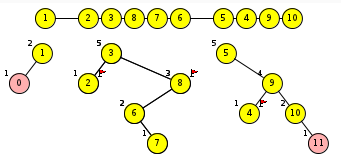
\includegraphics[width=\columnwidth]{obrazky/rev3trees.png}
\caption{\emph{Tri stromy.} Pri operácii \reverse\ sa strom rozdelí na 3 stromy. 
Vľavo prvky pred intervalom, vpravo prvky za ním. 
Na reverznutie intervalu stačí dať vlajku koreňu stredného stromu.}
\label{img:rev2}
\end{figure}

Pri takomto riešení musíme ešte upraviť vyhľadávanie a rotácie, aby brali do úvahy vlajky vo vrcholoch.
Najelegantnejšie riešenie je odstrániť vlajku vždy, keď na ňu narazíme:
Danému vrcholu odstránime vlajku, vymeníme mu synov a každému synovi vlajkový bit znegujeme.

Všetky operácie vieme implementovať v rovnakom čase ako operácie v splay tree, teda amortizovaná 
časová zložitosť oboch operácií je $O(\log n)$.

\paragraph{Použitie.}
Stromy s reverzami (pôvodne založené na AVL stromoch) navrhli \citet{chrobak}
na efektívnu implementáciu 2-opt heuristiky na riešenie problému obchodného cestujúceho.
Pri 2-opt heuristike sa snažíme reverzovať úseky cesty, kým nenájdeme lokálne minimum.

V bioinformatike sa tieto stromy používajú na triedenie orientovaných permuácií
pomocou reverzov \citep{reversals,reversals2}.

Za povšimnutie stojí fakt, že táto dátová štruktúra podporuje výmenu ľubovoľných dvoch blokov
v logaritmickom čase, keďže túto operáciu vieme odsimulovať pomocou štyroch reverzov.

\paragraph{Vizualizácia.}
Pre lepšiu vizualizáciu sme pridali do stromu nultý a posledný prvok. Tieto prvky
do reverzovateľného intervalu nepatria, majú však zmysel v prípade, ak sa reverzuje
interval, ktorý zahŕňa aspoň jeden okraj. V tom prípade v operácii \reverse\ nezostane
ani $T_1$ ani $T_3$ prázdny. Aby nevznikli problémy s operáciami, za krajné kľúče boli
zvolené hodnoty $0$ a číslo o jedna väčšie od aktuálneho maxima. Zároveň, pre lepšiu
predstavu, bolo pridané pole, v ktorom užívateľ vidí skutočné poradie prvkov, ktoré
zo stromu nie je až tak zjavné (obr.~\ref{img:rev1}). Pole simuluje operácie spolu so stromom, ale tie sú
na ňom vykonávané v lineárnom čase.

\begin{figure}
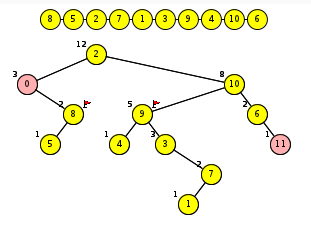
\includegraphics[width=\columnwidth]{obrazky/reversal.png}
\caption{\emph{Strom s reverzami.} Pre ľudí je názornejšie pole, počítaču viac vyhovuje strom.}
\label{img:rev1}
\end{figure}
